%\documentclass{sig-alternate}
\documentclass[conference]{IEEEtran}

\usepackage[bookmarks=false, urlcolor=black, linkcolor=black, citecolor=black, colorlinks=true]{hyperref}

\usepackage{graphicx}
\usepackage{pifont}
\usepackage{url}
%\usepackage{code}
\usepackage{amsmath}
\usepackage{amssymb}
\usepackage{caption}
\usepackage{algorithm}
\usepackage{multicol}
\usepackage{pgfplots}
%\usepackage{fontspec}
\usepackage{xspace}
\usepackage{fancybox}
\usepackage{code}

\newcommand{\note}[1]{\fbox{\parbox{0.8\linewidth}{\color{red} #1}}}


\usepackage{algpseudocode}
\usepackage{listings}
\usepackage{xcolor}
\usepackage{comment}

\lstdefinestyle{BashInputStyle}{
  language=java,
  basicstyle=\small\sffamily,
  numbers=left,
  numberstyle=\tiny,
  numbersep=3pt,
  frame=tb,
  linewidth=0.9\linewidth,
  xleftmargin=0.1\linewidth
}


\definecolor{dkgreen}{rgb}{0,0.6,0}
\definecolor{gray}{rgb}{0.5,0.5,0.5}
\definecolor{mauve}{rgb}{0.58,0,0.82}

\lstset{frame=tb,
  language=Java,
  aboveskip=3mm,
  belowskip=3mm,
  showstringspaces=false,
  columns=flexible,
  basicstyle={\small\ttfamily},
  numbers=none,
  numberstyle=\tiny\color{gray},
  keywordstyle=\color{blue},
  commentstyle=\color{dkgreen},
  stringstyle=\color{mauve},
  breaklines=true,
  breakatwhitespace=true,
  tabsize=3
}


%\newcommand{\comment}[1]{}

% correct bad hyphenation here
\hyphenation{op-tical net-works semi-conduc-tor}

\newcommand\mytool{hddRASS\xspace}
\newcommand\mytitle{Building Resource Adaptations via Test-Based Software Minimization: Application, Challenges, and Opportunities}

\newcommand\RASS{\emph{RASS}\xspace}
\newcommand\HDD{\emph{hierarchical delta debugging}\xspace}
\newcommand\sofs{sacrificability of specifications\xspace}

\newcommand\IMU{$M^{+}$\xspace}
\newcommand\AIMU{mean $M^{+}$\xspace}

\begin{document}
%
% paper title
% Titles are generally capitalized except for words such as a, an, and, as,
% at, but, by, for, in, nor, of, on, or, the, to and up, which are usually
% not capitalized unless they are the first or last word of the title.
% Linebreaks \\ can be used within to get better formatting as desired.
% Do not put math or special symbols in the title.
\title{ \mytitle}


% author names and affiliations
% use a multiple column layout for up to three different
% affiliations
\author{
\IEEEauthorblockN{Arpit Christi}
\IEEEauthorblockA{School of Computing\\
Weber State University\\
Ogden, UT, USA\\
arpitchristi@weber.edu}
\and
\IEEEauthorblockN{Alex Groce}
\IEEEauthorblockA{School of Informatics, Computing, and Cyber Systems\\
Northern Arizona University\\
Flagstaff, AZ, USA\\
agroce@gmail.com}
\and
\IEEEauthorblockN{Austin Wellman}
\IEEEauthorblockA{Raytheon BBN \\
\\
Boston, MA, USA\\
austin.wellman@raytheon.com}
}

%CISPA Helmholtz Center for Information Security Stuhlsatzenhaus 5 Saarbrücken, Saarland 66123 Germany rahul.gopinath@cispa.saarland


% conference papers do not typically use \thanks and this command
% is locked out in conference mode. If really needed, such as for
% the acknowledgment of grants, issue a \IEEEoverridecommandlockouts
% after \documentclass

% for over three affiliations, or if they all won't fit within the width
% of the page, use this alternative format:
% 
%\author{\IEEEauthorblockN{Michael Shell\IEEEauthorrefmark{1},
%Homer Simpson\IEEEauthorrefmark{2},
%James Kirk\IEEEauthorrefmark{3}, 
%Montgomery Scott\IEEEauthorrefmark{3} and
%Eldon Tyrell\IEEEauthorrefmark{4}}
%\IEEEauthorblockA{\IEEEauthorrefmark{1}School of Electrical and Computer Engineering\\
%Georgia Institute of Technology,
%Atlanta, Georgia 30332--0250\\ Email: see http://www.michaelshell.org/contact.html}
%\IEEEauthorblockA{\IEEEauthorrefmark{2}Twentieth Century Fox, Springfield, USA\\
%Email: homer@thesimpsons.com}
%\IEEEauthorblockA{\IEEEauthorrefmark{3}Starfleet Academy, San Francisco, California 96678-2391\\
%Telephone: (800) 555--1212, Fax: (888) 555--1212}
%\IEEEauthorblockA{\IEEEauthorrefmark{4}Tyrell Inc., 123 Replicant Street, Los Angeles, California 90210--4321}}




% use for special paper notices
%\IEEEspecialpapernotice{(Invited Paper)}




% make the title area
\maketitle


\begin{abstract}

Building resource adaptive software systems is a challenging problem. Researchers have proposed many techniques and tools to build such systems. We previously proposed a technique called Test-based Software Minimization (TBSM) that relies on using tests to define functionality that can be sacrificed to achieve resource gain. We demonstrate easy-applicability, usability, and effectiveness of TBSM by building resource adaptations for two real-world scenarios. We also discover significant challenges associated with the practical application of TBSM. Based on our attempt to overcome the challenges for two scenarios, we summarize possible solutions to the challenges, and note that these solutions are synergistic with a larger goal of improving software quality.

\end{abstract}

\section{Introduction}

Ultra Large-Scale Systems, Internet of Things applications, and Cyber-Physical Systems face increased resource variability compared to programs of the past, with real-world physical consequences.  Resources may be explicit: e.g., CPU, memory, or storage; or they may be implicit, e.g., libraries and protocols. The inability of software to handle resource changes effectively and automatically can produce inferior or potentially vulnerable systems~\cite{hughes2016building}. 

Self-Adaptive Software Systems (SAS) modify their own behavior in response to changes in operating conditions. Resource Adaptive Software Systems (RASS) are a subset of SAS where the trigger for adaptation is variability or unavailability of resources. For longevity and survivability of modern systems, self-adaptation for resource changes is essential: hence the problem of self-adaptation is well studied~\cite{seams2018keynote}. To this end, DARPA started the BRASS (Building Resource Adaptive Software Systems) program, a major initiative to bring researchers and practitioners together to solve the problem of building resource adaptive software. 

Researchers have proposed many techniques, approaches, and tools to build SAS automatically~\cite{hughes2016building,salehie2009selfadaptive,krupitzer2015a}. We previously proposed a solution called Test-Based Software Minimization (TBSM) to build SAS to overcome some of the limitations of previous approaches based on our work with Raytheon developers as part of BRASS~\cite{christi2017saso}. In this work, we applied TBSM to produce adaptations of a mission-critical military system and the popular NetBeans \texttt{Java} IDE.  Based on our observations: 
\begin{enumerate}
\item {We demonstrate that unlike most other previous approaches, resource adaptation via TBSM is a conceptually simple, usable, and applicable technique. }
\item {We present challenges we faced while attempting to produce accurate resource adaptations automatically. }
\item {We present the solutions we employed to solve some of those challenges. }
\item {We explore a synergy between some of the solutions to the problems of TBSM and the problems of reliable software development.}
\end{enumerate}

In the process, we identify opportunities to further aid developers in effectively employing test-based minimization to achieve resource adaptations. 








\section{Background}
\label{ref:background}
\begin{figure*}
\begin{center}
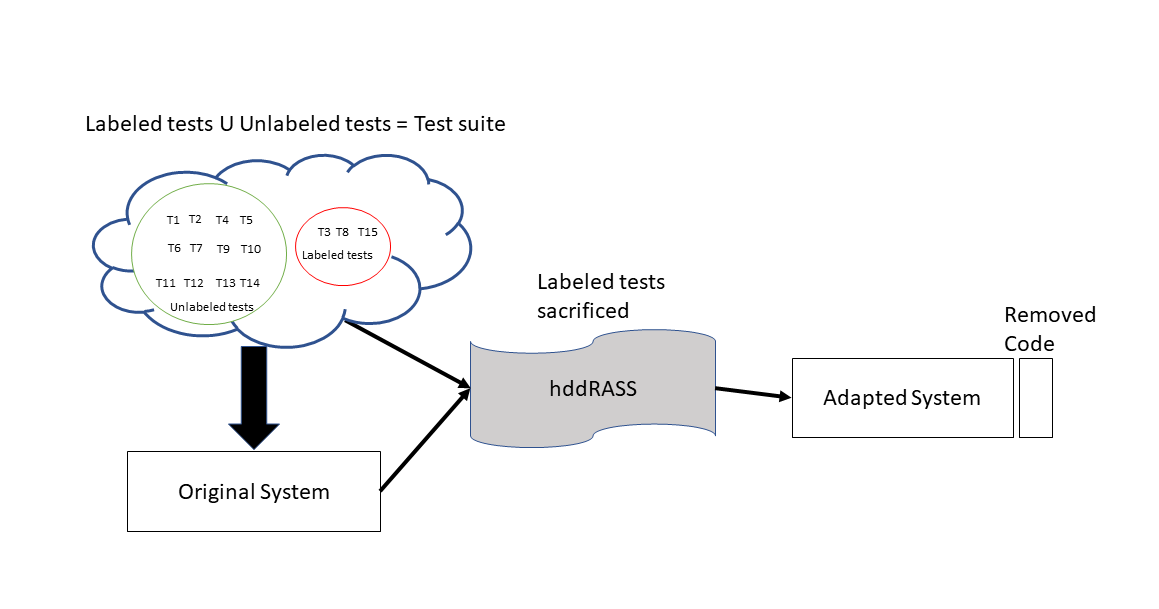
\includegraphics[scale = 0.50]{icst_19_fig1.png}
\caption{TBSM approach to build adaptation for single adaptation objective
scenario. Labeled tests encode adaptation specification for single resource
variability.}
\label{fig:workflow}
\end{center}
\end{figure*}

While working with developers attempting to build SAS for a real-world, mission-critical system, we observed that (1) most developers speak the language of tests fluently, unlike that of formal methods or architectural descriptions,  (2) tests are thus, for most complex projects in the real world, the \emph{only} semi-formal specification available. To exploit both the widespread availability of tests for mission-critical systems and developers' familiarity with tests, we proposed capturing resource adaptation specifications using tests.
TBSM relies on developers' understanding of tests, and how tests relate to program features and resource usage. Developers encode this information by simply labeling the tests. Test labels can be a multi-dimensional space in feature, resource, and priority. To demonstrate the concept, we assume a single adaptation objective: a single resource faces variability or unavailibility. The concept is demonstrated in Fig.~\ref{fig:workflow} (a simplified version of Fig 2. in the original paper proposing TBSM~\cite{christi2017saso}. We reuse this figure from our previous work to keep the paper self-contained.~\cite{christi2019qrs}). Labeled tests define functionality that can be sacrificed to reduce resource usage. Unlabeled tests define the functionality that is to be retained and not modified. A tool called hddRASS takes as its input the test suite with labeled and unlabeled tests and the original program, and produces a minimized program such that the functionality marked by labeled tests is removed. hddRASS achieves this by temporarily removing the labeled tests from the suite and using the Hierarchical Delta Debugging (HDD) algorithm to find a minimal program, such that retained tests continue to pass~\cite{misherghi2006hdd}. The basic idea is that if the labeled tests define a functionality that uses resources, removing that functionality will ensure resource adaptation. TBSM builds adaptations, in a sense, in the same way that Automatic Program Repair fixes faults. In APR, the goal is to modify the program to pass a set of previously failing tests (without failing previously passing tests)~\cite{monperrus2018asr}. In TBSM, the goal is to modify the program while removing as much code as possible, while still passing a set of unlabeled tests.



\section{Case Study}
Building an adaptive software system is not (yet) a common practice. The example benchmarks available as part of self-adaptive exemplars are unfortunately not applicable to TBSM, due to the nature of their tests and the resources adapted~\cite{exemplars}. Hence, we rely on two real-world case studies.   

We worked with a group of developers attempting to build adaptations for a mission-critical system called the Tactical Situational Awareness System (TSAS). To focus our discussion, we present one adaptation scenario, the \textit{Elevation API} scenario. The resource under consideration is a library (an implicit resource) that has been updated to a new version. Developers labeled tests in terms of the feature tested. Certain features were marked as sacrificial (able to be ``sacrificed'', i.e., removed) because the new version of the library provides functionality that was originally part of the TSAS code, the functionality these features was intended to provide. The sandboxed TSAS version that we used consists of 70 \texttt{Java} files, with 5,571 LOC, and developers labeled 5 tests as representing sacrificial functionality; the remaining tests were considered unlabeled. The developers used TBSM/hddRASS to build an adaptation.

For our next case study, we used the popular \textit{NetBeans IDE} for \texttt{Java}. We discussed the \textit{NetBeans IDE} case study in detail in our original work~\cite{christi2017saso}. The resource under consideration in this case was memory. To save memory, we adapted the IDE by disabling undo-redo functionality, which is potentially memory-intensive. Developers working in a memory-limited setting would prefer to lose undo-redo rather than face constant crashes due to memory exhaustion. Our target for adaptation is the \texttt{openide.awt} module, which consists of 69 \texttt{Java} files, 11,284 LOC, and 146 tests. After carefully studying the code and tests we labeled 3 tests as undo-redo related. We then applied TBSM to build a memory adaptive \textit{NetBeans IDE}. As most of the 69 \texttt{Java} files are clearly not related to the undo-redo feature, we chose the two most likely files as reduction targets to reduce processing time~\cite{christi2017saso}. 


\section{Evaluation}
We evaluate resource adaptation via TBSM/hddRASS along several dimensions: effectiveness, usability, applicability, and scalability.

\subsection{Effectiveness}
For the \textit{Elevation API} scenario, all 4 necessary modifications were correctly performed automatically by TBSM. The development team was able to confirm the adaptations for the library update by (1) examining the code for necessary modifications (2) running the tests and (3) using the application. As TSAS is a proprietary system, we have to rely on conformation from the development team. All the necessary modifications to adapt the \textit{NetBeans IDE} were also performed correctly. We observe that all 19 resource consuming statements (as identified in previous work~\cite{christi2018qrs}), the statements that fill the undo-redo buffers, were correctly modified by the technique. We have shown previously that the adapted IDE 1) cannot perform undo-redo operations and 2) uses far less memory, in a controlled experiment setting allowing only edits to a single text file~\cite{christi2017saso}. We also confirm otherwise normal operation of the IDE.

\subsection{Usability}
Most adaptation approaches require developers to learn a new specification language or add complex annotations to code. To use such techniques, developers typically need to use modeling approaches, architectural specifications, formal methods, etc., to map their application to a view that the adaptation technique supports; this is obviously a time consuming and error-prone task~\cite{salehie2009selfadaptive, krupitzer2015a}. TBSM only requires developers to look at their tests and make a ``good guess'' about the feature(s)/resource(s) relevant to each test. Developers are familiar with tests and can likely perform this task without additional training. For the \textit{NetBeans IDE} case, it took us only a few hours to determine 3 tests to label out of 146 tests, despite the fact that we are not developers, or familiar with the NetBeans code in any way before we examined it. For the \textit{Elevation API}, actual developers were almost instantly able to determine the tests pertaining to certain features.

\subsection{Applicability}
While developing the RAINBOW framework, Garlan et al. noted that most previous approaches for SASS were scenario-based or application-specific, and not very reusable~\cite{garlan2004rainbow}. To evaluate applicability, we measured the effectiveness of hddRASS as a tool. We believe hddRASS to be complete for \texttt{Java} 7: it applies to any programs written in \texttt{Java} 7. To confirm this, we checked for thrown exceptions or unprocessed statements when minimizing real-world systems. While applying hddRASS to TSAS, we processed 70 \texttt{Java} files with 338 non-constructor methods. For the \textit{NetBeans IDE}, we processed 2 \texttt{Java} files with 38 non-constructor methods. We also applied hddRASS to 40 randomly selected classes with a total of 1,207 methods across 10 open source projects, using a random labeling scheme~\cite{christi2018qrs}. We observed neither exceptions nor unprocessed statements across these experiments. Based on this, we can say that hddRASS as a tool, and TBSM as a technique, is generally applicable to \texttt{Java} applications. To extend it to other programming languages, one needs to build hddRASS like tools for those languages.    

\subsection{Scalability}
For the \textit{Elevation API} the application of hddRASS, using no heuristics, on all 70 {\tt Java} files took 7 hours and 50 minutes. For \textit{NetBeans IDE}, adapting two files in \texttt{openide.awt} using no heuristics took 2 hours and 35 minutes. As the program size increases or test suite runtime increases, scalability becomes the limiting factor in TBSM. For offline adaptations, scalability may not be a problem; machine time is cheap, programmer time expensive. But for live systems deployed in the wild, the system needs to be halted until adaptations are performed and a long offline period is not normally acceptable.  The speed of the most thorough version of TBSM without heuristics to guide adaptation is likely acceptable for use before deployment, e.g., to prepare a specialized version of a system for a resource-limited platform, but unsuitable for field use.  However, as we discuss below, even without additional developer effort, use of heuristics to compute approximate or incremental best-effort adaptations can mitigate this problem substantially.


\section{Challenges}
We describe the major challenges that we faced while applying TBSM to build real-world RASS, and how we attempted to solve these challenges for the case study scenarios. In the process, we identify major research challenges in TBSM. We note the similarity between the challenges in TBSM and the challenges observed by researchers in APR~\cite{LeGoues2013}.

\subsection{Search Space}
TBSM indiscriminately processes all the statements of a program, so the search space is accordingly vast. This can be significantly reduced by selecting only statements likely to actually be modified. We empirically evaluated a large number of adaptation related modification for 800 synthetic adaptations to derive heuristics to guide target selection. We derived statistics-based heuristics (H1, H2) and dynamic-analysis-based heuristics (CBLS, AdFL) based on our evaluation~\cite{christi2018qrs,christi2019qrs}. The CBLS heuristic relies on coverage information for thelabeled and unlabeled test suite. We repurpose Spectrum-Based Fault Localization (SBFL) to derive the more general AdFL heuristic by establishing equivalence between core components of SBFL and core components of TBSM. We found that dynamic-analysis-based heuristics  perform better in empirical analysis. For the \textit{Elevation API} scenario, CBLS reduces the search space by 55\% and AdFL heuristics reduces search space by 92\% bringing the wall clock time to build adaptations down from 460 minutes to 118 minutes for CBLS and 49 minutes for AdFL.  For the \textit{NetBeans IDE} scenario, CBLS heuristics reduces search space by 90\% and AdFL heuristics reduces search space by 94\% bringing the wall clock time down from 175 minutes to 61 minutes and 57 minutes for CBLS and AdFL respectively. 

The CBLS heuristics provides search space reduction while AdFL prioritizes the search space based on likeliness of modification. We demonstrated that the likely targets of modifications would appear earlier in the sorted order if we use AdFL~\cite{christi2019qrs}. We used this fact to circumvent the search space issue all together. We proposed best-effort incremental TBSM as a technique were developers provide a time limit to finish the adaptations~\cite{christi2019qrs}. The best-effort incremental TBSM will always produce a useable system in the given amount of time, with resource adaptation achieved entirely or partially. For \textit{Elevation API} and \textit{NetBeans IDE} scenarios, time limits of 35 minutes and 20 minutes, respectively, were sufficient to perform complete resource adaptation using best-effort incremental TBSM. Best-effort incremental TBSM performs better than AdFL heuristics with 90\% search space reduction for both scenarios. 

\subsection{Test Suite Runtime }
Like APR, TBSM is a generate-and-validate technique that must execute a potentially large test suite to evaluate each modification. TBSM benefits from a large test suite, but running all tests is often prohibitively slow. The version of \textit{NetBeans IDE} we used has a test suite that requires 7+ hours to run for all 1193 modules. TSAS also exhibits unacceptably slow complete test suite runtime. For both case studies, we observe that running only modified-module-related tests is sufficient, as modules are self-contained and have good individual test suites. We observe that even such a simple ad-hoc test selection reduces test runtime to 34 seconds and 18 seconds for the \textit{NetBeans IDE} and \textit{Elevation API}, respectively. For most resource adaptation scenarios, such an ad-hoc technique is not feasible and scalable. We need test selection and prioritization (since early failures also limit runtime) tailored to TBSM.

\subsection{Inefficient Algorithm}
Our hddRASS reducer uses a modified HDD$^*$ algorithm with worst-case running time of $O(n^3)$, where $n$ in our case is the number of statement nodes of the abstract syntax tree of the program~\cite{misherghi2006hdd}. We employ HDD$^*$ as the underlying driver for TBSM because it guarantees convergence and minimality. By minimality, we mean that any output program produced by TBSM is minimal and cannot be modified any further. One solution we employ is to forgo the minimality guarantee of HDD$^*$ and use a pure greedy search, trading accuracy for efficiency.  With a greedy search strategy, we can build resource adaptations 1.72 times faster while retaining 94\% accuracy for the \textit{Elevation API} and 1.90 times faster while retaining 100\% accuracy for \textit{NetBeans IDE}. We need further evaluation of different search strategies and heuristics-based modifications to HDD$^*$.

\subsection{Overfitting}
The issue of overfitting is well studied in APR, and we face the same problem\cite{smith2015cwd}. TBSM produces test-adequate adaptations, adaptations that are correct with respect to a test suite and test labeling scheme. For our case studies, Type 1 errors are rare, and even related statements are usually removed; e.g., if a single resource consuming statement is the body of a for loop, the loop is removed as well. We consider directly or indirectly resource-adaptation-related modifications as correct modifications. We do observe a large number of false modifications, modifications that are not directly or indirectly related to resource adaptations: these are the more common Type 2 errors. Indeed, the false modifications outnumber true ones in our scenarios. A total of 49 and 121 modifications are performed by TBSM for the \textit{Elevation API} and \textit{NetBeans IDE} scenarios, respectively. We observe 91\% and 51\% false modification rates for the \textit{Elevation API} and \textit{NetBeans IDE} adaptations, respectively. As TBSM generated test-adequate adaptations overfit a given test suite and labeling scheme, TBSM is vulnerable to both (1) inadequacy of the test suite and (2) labeling errors. Developers reported instances where TBSM-generated modifications removed untested but desired functionality. 

\section{Test Adequacy and Adaptation Quality}
Developers using TBSM expressed more concern over overfitting than any other problem.  In this section we note the origins of this problem, and propose that solving it is synergistic with addressing a long-standing problem in software development.

\subsection{Test Inadequacy}

TBMS only knows what the tests tell it.  If tests are grossly inadequate, it is bound to produce sub-standard adaptations; in particular, TBSM is aggressive, and if a test does not force the inclusion of code in the adapted program, TBSM is likely to remove that functionality.  There are two basic sources of inadequacy.  One is true inadequacy, where the feature that TBSM ``accidentaly'' removes is simply not tested at all.  The solution to this problem is to test all features of a system that are of any actual importance, a worthy goal in any case.  The second problem is that there may be some tests for a feature, but they are all mixed-in with tests for a feature that is to be removed.  That is, the tests for a system are not well decomposed, and some functionality is only tested in conjunction with a feature that a developer wants to ``adapt away.''  Fortunately, these problems can be addressed by taking a better approach to tests in general.

\subsection{Code Coverage} 
TBSM will remove any code that is not covered by any tests, and not required for compilation. The easiest way to avoid this problem is to start with a high-coverage, high-quality test suite. Developers can target poorly covered code with manual tests or use targeted test generation tools to cover such code. Improving code coverage using random testing reduced overfitting by 23\% and 8\% for \textit{Elevation API} and \textit{NetBeans IDE} respectively. Na\"ive test generation will not necessarily improve matters, however. Developers have to label any generated tests, and if tests mix multiple features, there still may often be cases where a feature not to be removed is never tested in isolation. We propose using delta-debugging, in particular \emph{cause reduction} to help isolate features in generated test cases~\cite{stvrcausereduce}: if a generated test covers two features, perhaps one can be removed by reducing the test with respect to targeted code for one feature only.  In fact, in principle, we can automatically take each individual line of code, and produce a test whose only purpose is to cover that line of code, with any other behavior required to retain that coverage.  If developers can then label files or functions in a program by functionality, the targeted code's location can automatically provide a label.

\subsection{Better Tests} 
Based on our study (with the developers) of overfitting, we identified a few categories covering most of the incorrect removals. For the \textit{Elevation API}, there were no tests for logging, and so all {\tt LOG} statements were removed. This problem is likely very common, but can be easily remedied by explicitly testing system logging as a feature.  Testing the logging output for performed actions in the tests for the functionality is a seldom-performed, but likely beneficial practice.  Similarly, exception-handling code was often inadequately tested.

We worked with the developers to produce a new test covering each major overfitting category identified. We produced just three and four (relatively small) tests, respectively, for the \textit{Elevation API} and \textit{NetBeans IDE} scenarios, resulting in 20\% and 66\% reduction in overfitting. Identifying overfitting categories can be a highly context-specific task, but we suspect new automated test generation methods targeting specific under-tested categories such as logging and exception handling may be useful here.

\subsection{Motivating Better Tests}

Of course, the reason tests are inadequate in the first place is that developers did not produce extremely high-quality, fine-grained tests.  Developers often fail to test important functionality, perhaps on the grounds that it is ``only logging'' (despite the fact that logging is, in the long run, the only visibility and debugging aid for many systems).  More seriously, even developers of high-quality systems may not test certain exceptional behavior paths.  Targeting often-overlooked functionality is a good future goal for the automated testing community; perhaps logging code is not tested because developers expect to change logging output frequently in reponse to debugging needs, and don't want to change the tests.  Automated methods could generate (and re-generate) properly labeled tests just to test the logging output of existing unit or system tests, without making this a significant burden on developers.  Aggressive random testing and fuzzing is likely to expose untested exceptional scenarios.  Interestingly, TBSM can also be seen as a way to identify untested code:  just run TBSM on a code base with \emph{no} labeled tests.  Anything removed is a good candidate for additional testing!

But there is a larger picture here.  We suspect that developers do not put as much effort as TBSM would ideally expect into testing because the payoff of testing is not always clear.  The relationship between test quality, even measured by mutation testing rather than coarse-grained coverage only, and detection and anticipation of important defects worth fixing, is not always extremely strong~\cite{Testedness}.  However, there is clearly some relationship between test quality and eventual system reliability, and one way to see TBSM (and future techniques of the same kind) is as a new way to get better tests.  Because most code does not have a critical bug, effort to write tests is currently seen as a burden, a ``cost-center,'' not a ``revenue-center'' for developers, to adapt a business analogy.  It may have to be done, but testing is purely to ward off disaster.  However, TBSM offers a different way to look at tests:  high quality tests allow developers to be more productive, in that they enable the \emph{automation of certain kinds of changes to the software.}  Writing high-quality tests may become a much more pleasant part of software development if the payoff is not having to write as much complex code to, e.g., adapt a system to a more limited platform, or handle changes to system libraries, or produce a more secure version with a smaller attack surface due to removing insecure functionalities.  If tests can produce ``productivity revenue'' rather than simply allowing the detection of faults in previous productivity, they may be more valued, and receive more attention.  The upshot will be more reliable systems that are also easier to adapt to resource-limited situations.

\section{Tool and Data Availability}
The hddRASS tool is available at \url{https://github.com/amchristi/hddRASS}. It supports the baseline TBSM technique as well as heuristics guidance (H1, H2, CBLS, or AdFL). It also provides support to execute TBSM in greedy mode. As TSAS is a proprietary system, we cannot make its source code, test suite, or tests labels available. The NetBeans IDE (and hence \texttt{openide.awt} module) source code is available online. We also  provide the exact \texttt{openide.awt} module source code, test suite and test labels that we used at \url{https://github.com/amchristi/AdFL}. The same link contains 800 synthetic adaptation scenarios with source code, tests, and test labels for empirical evaluation and comparison. 



\section{Ongoing Work and Future Directions}
As part of DARPA BRASS project, we work with multiple software development teams and other collaborators. Our communication with these stakeholders as well as the feedback that we received from the development teams utilizing our work are driving our ongoing work and future research direction. 
\subsection{Ongoing Work}
\subsubsection{Improving Applicability}
The underlying tool hddRASS that drives TBSM is written for \texttt{Java} program only. Raytheon development team utilizes TBSM for TSAS, an application written in \texttt{Java}. We also developed a \texttt{C++} version of hddRASS that is intended to be used by ROS (Robotics Operating System) application developers to adapt against ROS version changes and other ROS package changes.  Developers can use it to build any different kind of resource adaptation for \texttt{C++} applications by providing correct test labeling. We plan to publish it soon. 

\subsubsection{Minimization vs Modification}
The primary concern that any development team might raise before evaluating TBSM to build resource adaptation is: It only offers minimization(reduction). When the software system adapts itself, the adaptation manifests itself in 3 ways (1) reduction (2) replacement (3) enhancement~\cite{hughes2016building}. The published TBSM version only supports reduction. While developing a \texttt{C++} version of hddRASS, we incorporated many other modification operators studied and used by APR to fix the fault, making few replacement capabilities available~\cite{Forrest2009genetic,Arcuri2009phdthesis,Debroy2010using}. We plan to continue to improve hddRASS to provide more modification capabilities. 

\subsection{Future Direction}
We are currently investigating multiple other ways to speed up TBSM, including using static and dynamic analysis to precompute the effects of program statements on test oracles and using test case selection and prioritization to reduce the running time of tests in TBSM’s generate-and-validate loop.

The original work in TBSM emphasized the need for a “good” test suite. Previous heuristics suggested coverage as a way to define “goodness” of a test suite; the CBLS heuristic depends on coverage information. Because of the success of AdFL heuristics in isolating and prioritizing modification targets, we plan to consider test suite diagnosability metrics as a more refined way to define the “goodness” of a test suite for TBSM, using approaches proposed by Baudry et al. and Perez et al.~\cite{Baudry2006improving,perez2017diagnosibility}

For our work, we mostly utilized existing test suites provided by the developers. For such test suites, we observe that sometimes a test that developer labeled as pertaining to a particular feature may contain code that exercises other features also. Similarly, an unlabeled test, apart from testing functionality that needs to be retained, may exercise sacrificial feature.  Availability of such tests makes it harder for TBSM to differentiate between an adaptation related modification and a pure accidental modification, resulting in underfitting or overfitting. To mitigate the situation, we plan to utilize (1) Test-case purification to segregate tests by features~\cite{xuan2014test} (2) Test-case reduction using delta debugger to remove irrelevant features from tests~\cite{stvrcausereduce,christi18reduce}.  

\section{Conclusions}
Test-based software minimization offers a conceptually simple, widely applicable, easily understood approach to generating resource adaptations. While TBSM faces significant scalability challenges, and cannot be applied where tests are impossible to label, or to resources not associated with removable features, it also benefits from a powerful synergy: namely, the best way to improve TBSM is to improve software test suites. Making test suites faster to execute, improving their granularity so that tests cover distinct features, increasing code coverage (and other test quality measures), and improving test prioritization techniques all lead not only to more efficient and effective TBSM, but to better fault detection and debugging.

{{\bf Acknowledgments}: this work was partly funded by the DARPA
  BRASS~\cite{hughes2016building} program, and the authors would like
  to thank our collaborators at Oregon State University and Raytheon/BBN.}


\bibliographystyle{IEEEtran}
% argument is your BibTeX string definitions and bibliography database(s)

\def\IEEEbibitemsep{0.6pt plus 0.9pt}

\bibliography{IEEEabrv,bibliography}

\end{document}
